
\section{Case studies}

\subsection{Routine characterization of a MOF sample}

The UiO-66(Zr) MOF and its derivatives are well known due to their thermal and chemical 
stability~\cite{cavkaNewZirconiumInorganic2008}. It is composed of
\ce{[Zr6O4(OH)4]^12+} clusters which are connected with benzene dicarboxilate (BDC) linkers to form
a face-centered cubic framework. It has shown promise~\cite{wiersumEvaluationUiO66GasBased2011}
in use for gas adsorption and catalytic applications.

When a newly synthesised sample is available, an initial characterisation is often performed
to compare the material with previous batches. Adsorption of nitrogen at \SI{77}{\kelvin}
is commonly used to verify if predictors such as specific surface area and pore size 
distribution are consistent with other samples or literature values. 

The nitrogen isotherm is first imported in \texttt{pyGAPS}. To obtain the BET 
area, the \lstinline{pygaps.area_BET()} method is used with the isotherm object as the 
parameter and the \lstinline{verbose} option, with Figure~\ref{fig:uiobet} as the output.
It can be seen that the framework has automatically selected the points within the 
applicable BET region using the checks devised by Rouquerol et al.
\cite{rouquerolAdsorptionPowdersPorous2013} to assert method validity. 
The statistical BET monolayer point is within
the selected region, which is one of the checks implemented for method validity.
The calculated surface area is \SI{1277}{\metre^2\per\gram}, which is similar to
literature values~\cite{wiersumEvaluationUiO66GasBased2011, 
valenzanoDisclosingComplexStructure2011}.

\begin{figure}[ht]
    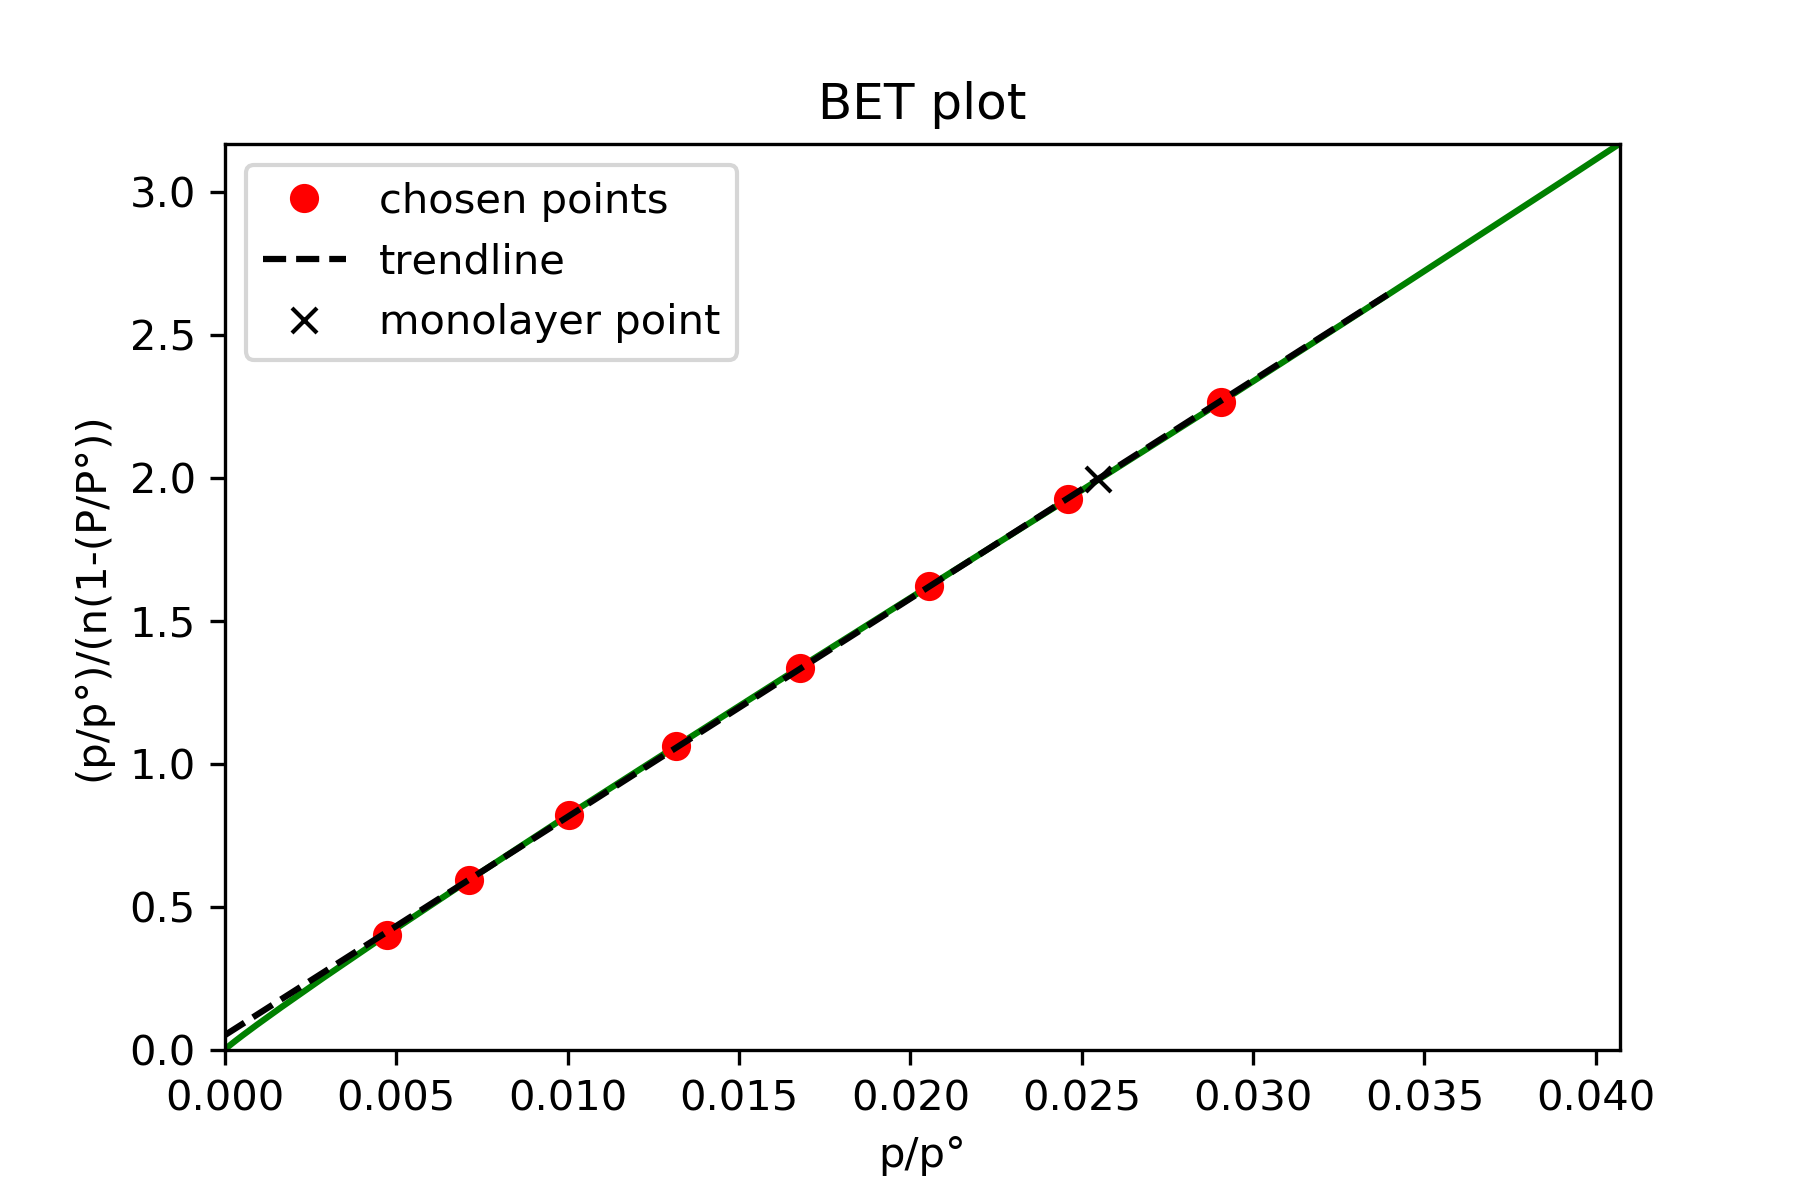
\includegraphics[width=\textwidth]{uio-bet}
    \caption{BET transformation and point selection}%
    \label{fig:uiobet}
\end{figure}

The same isotherm is used to calculate the pore size distribution of the UiO-66(Zr) sample.
This MOF has octahedral cages surrounded by eight corner 
tetrahedral cages of 11 and 8 \si{\angstrom} respectively. 
The structure is therefore expected to have only 
micropores. Two methods are available in \texttt{pyGAPS} for micropore size distributions:
a `classical' Horvath-Kawazoe (HK) method~\cite{horvathMethodCalculationEffective1983}, 
as well as a DFT fitting routine.
The HK method is called by using the function in Listing~\ref{lst:PSD}.
Here, the surface characteristic parameters determined by Saito and 
Foley~\cite{saitoCurvatureParametricSensitivity1991} are to
be used, with the framework automatically supplying the parameters for the adsorbed gas. 

\begin{lstlisting}[caption={Calculating the PSD},label={lst:PSD}]
pygaps.micropore_size_distribution(iso, 
                                   psd_model='HK', 
                                   adsorbent_model='OxideIon(SF)')
pygaps.dft_size_distribution(iso, kernel_path='internal')
\end{lstlisting}

The DFT fitting is done using the internal kernel
which is applicable for \ce{N2} on carbon slit pores and included with \texttt{pyGAPS}. 
Results are shown in Figure~\ref{fig:uiopsd}. We can see that whilst both methods
produce a bimodal size distribution, neither is accurate in describing the crystallographic pore
widths. This is to be expected, since neither method is applicable to the UiO-66(Zr)
system. However, when comparing two samples of the same MOF, these methods can still
highlight differences in the quality of the two batches. For example, it can be seen
that the DFT method shows wide peaks at >\SI{1}{\nano\meter}
which can be an indication of the presence of defects in the UiO-66(Zr) structure.
Indeed, TGA analysis of the pristine sample shows a linker ratio (11.8 linkers per cluster)
that is lower than it would be in a perfect sample (see figure in supplemental information.) 

\begin{figure}[ht]
    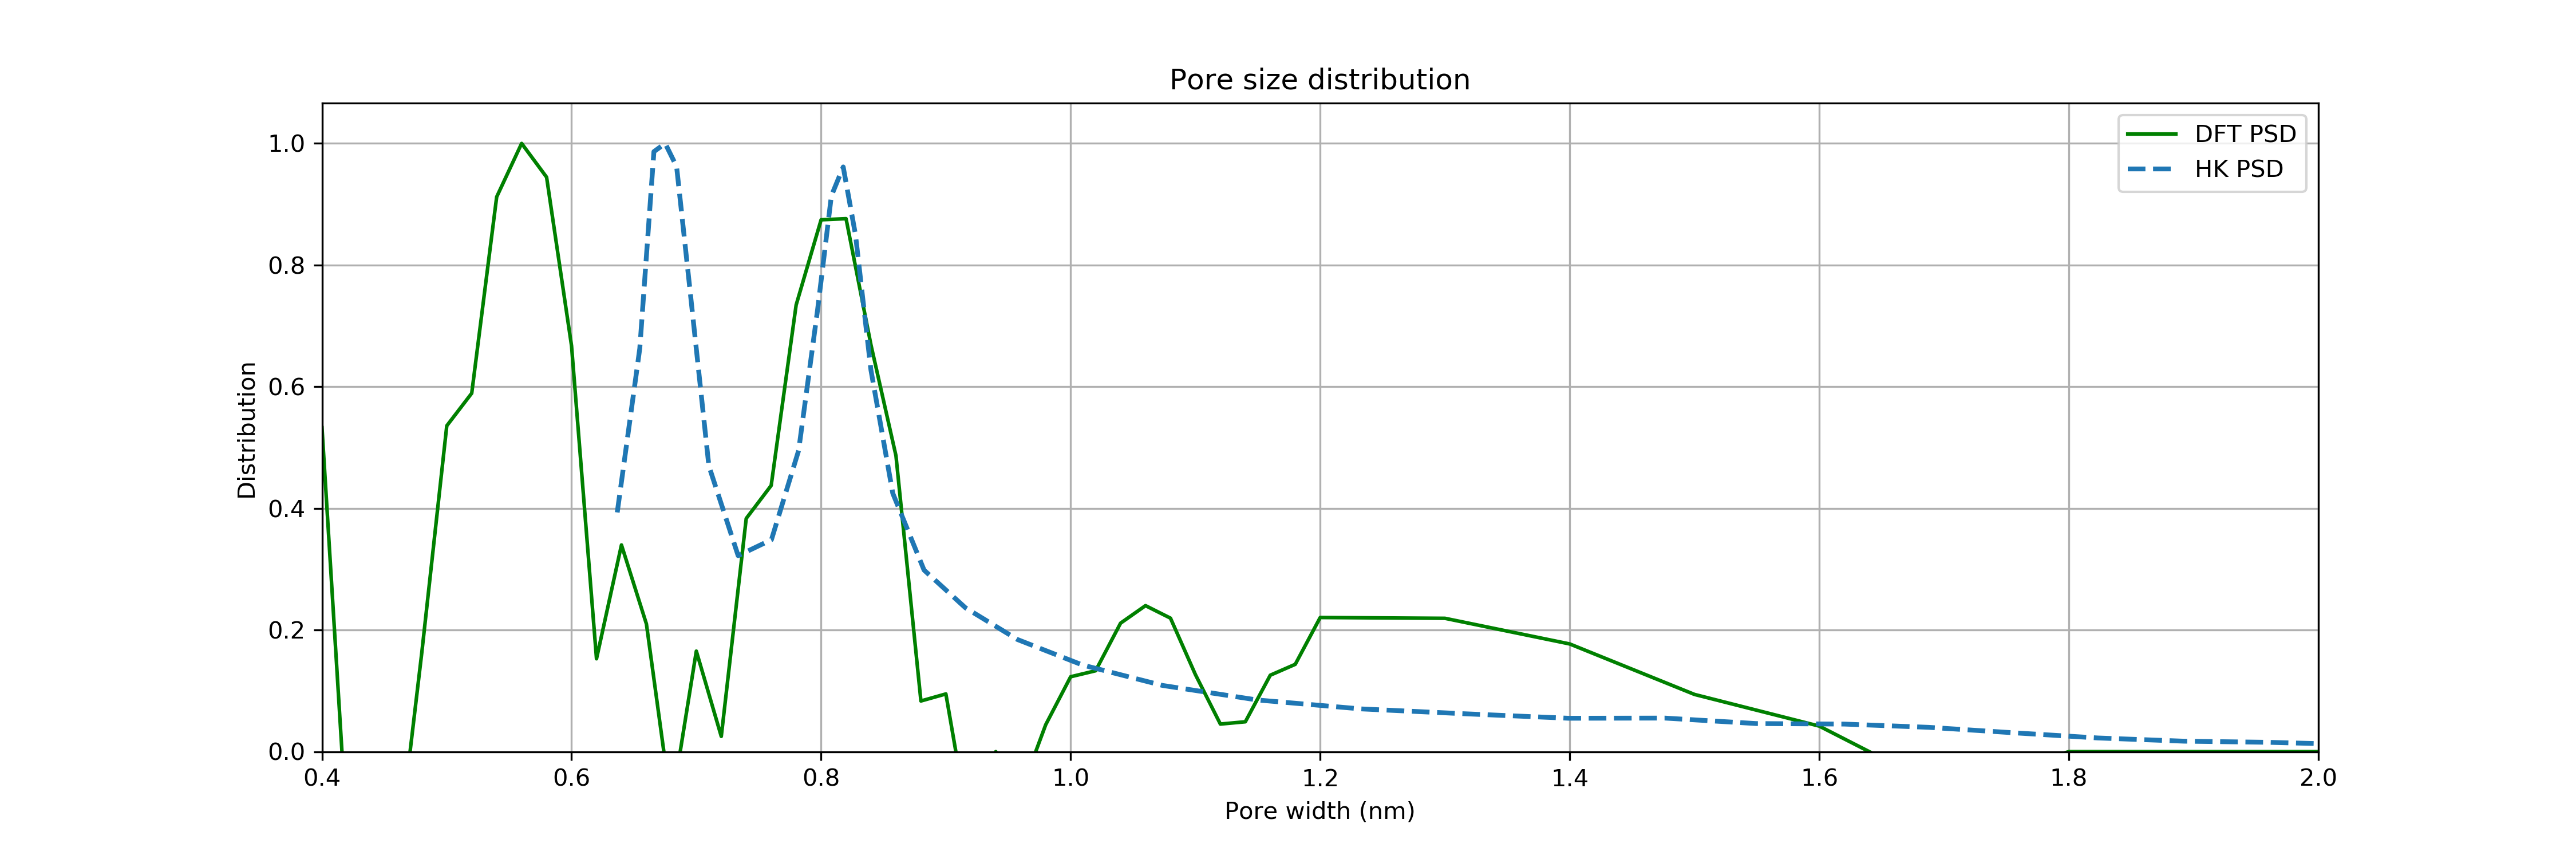
\includegraphics[width=\textwidth]{uio-psd}
    \caption{Pore size distribution calculated through the Horvath-Kawazoe method (dotted 
    blue line) and the internal DFT kernel (continuous green line)}%
    \label{fig:uiopsd}
\end{figure}

New materials are often screened for their ability to act as a \ce{CO2} capture material. 
A good predictor of performance 
in this application are the enthalpies of adsorption, which are an indication of
host-guest interactions. Here, we first measure the differential heats of adsorption
directly through the use of adsorption microcalorimetery at \SI{303}{\kelvin}. 
Then, to determine the isosteric heats of adsorption,
two isotherms have been measured at \SI{303}{\kelvin} and \SI{323}{\kelvin} respectively. 
The complete set of isotherms is loaded into \texttt{pyGAPS} and plotted by the 
\lstinline{pygaps.plot_iso()} function as seen in Figure~\ref{fig:uioisostericiso}. 
To calculate the isosteric heat
of adsorption, the two isotherms measured for this purpose are passed through the 
\lstinline{pygaps.isosteric_heat()} function. The results from the calculation are overlaid 
on top of the measured calorimetric data in 
Figure~\ref{fig:uioisostericheat}. The two datasets are
overlap for the most part but diverge at low loadings and near complete coverage.
At low loading the small changes in pressure amount introduce large errors in the 
Clausius-Clapeyron equation. This, together with the breakdown of the 
assumption of equilibrium due to active sites in the MOF lead to the calorimetric
measurement providing more valid results. At higher loadings, where the isotherm reaches
a plateau and the change in adsorbed amount is small from point to point, errors are
introduced in the direct calculation of the heat of adsorption. The two techniques are thus 
complementary.  

\begin{figure}[ht]

    \centering
    \begin{subfigure}[b]{.5\textwidth}
        \centering
        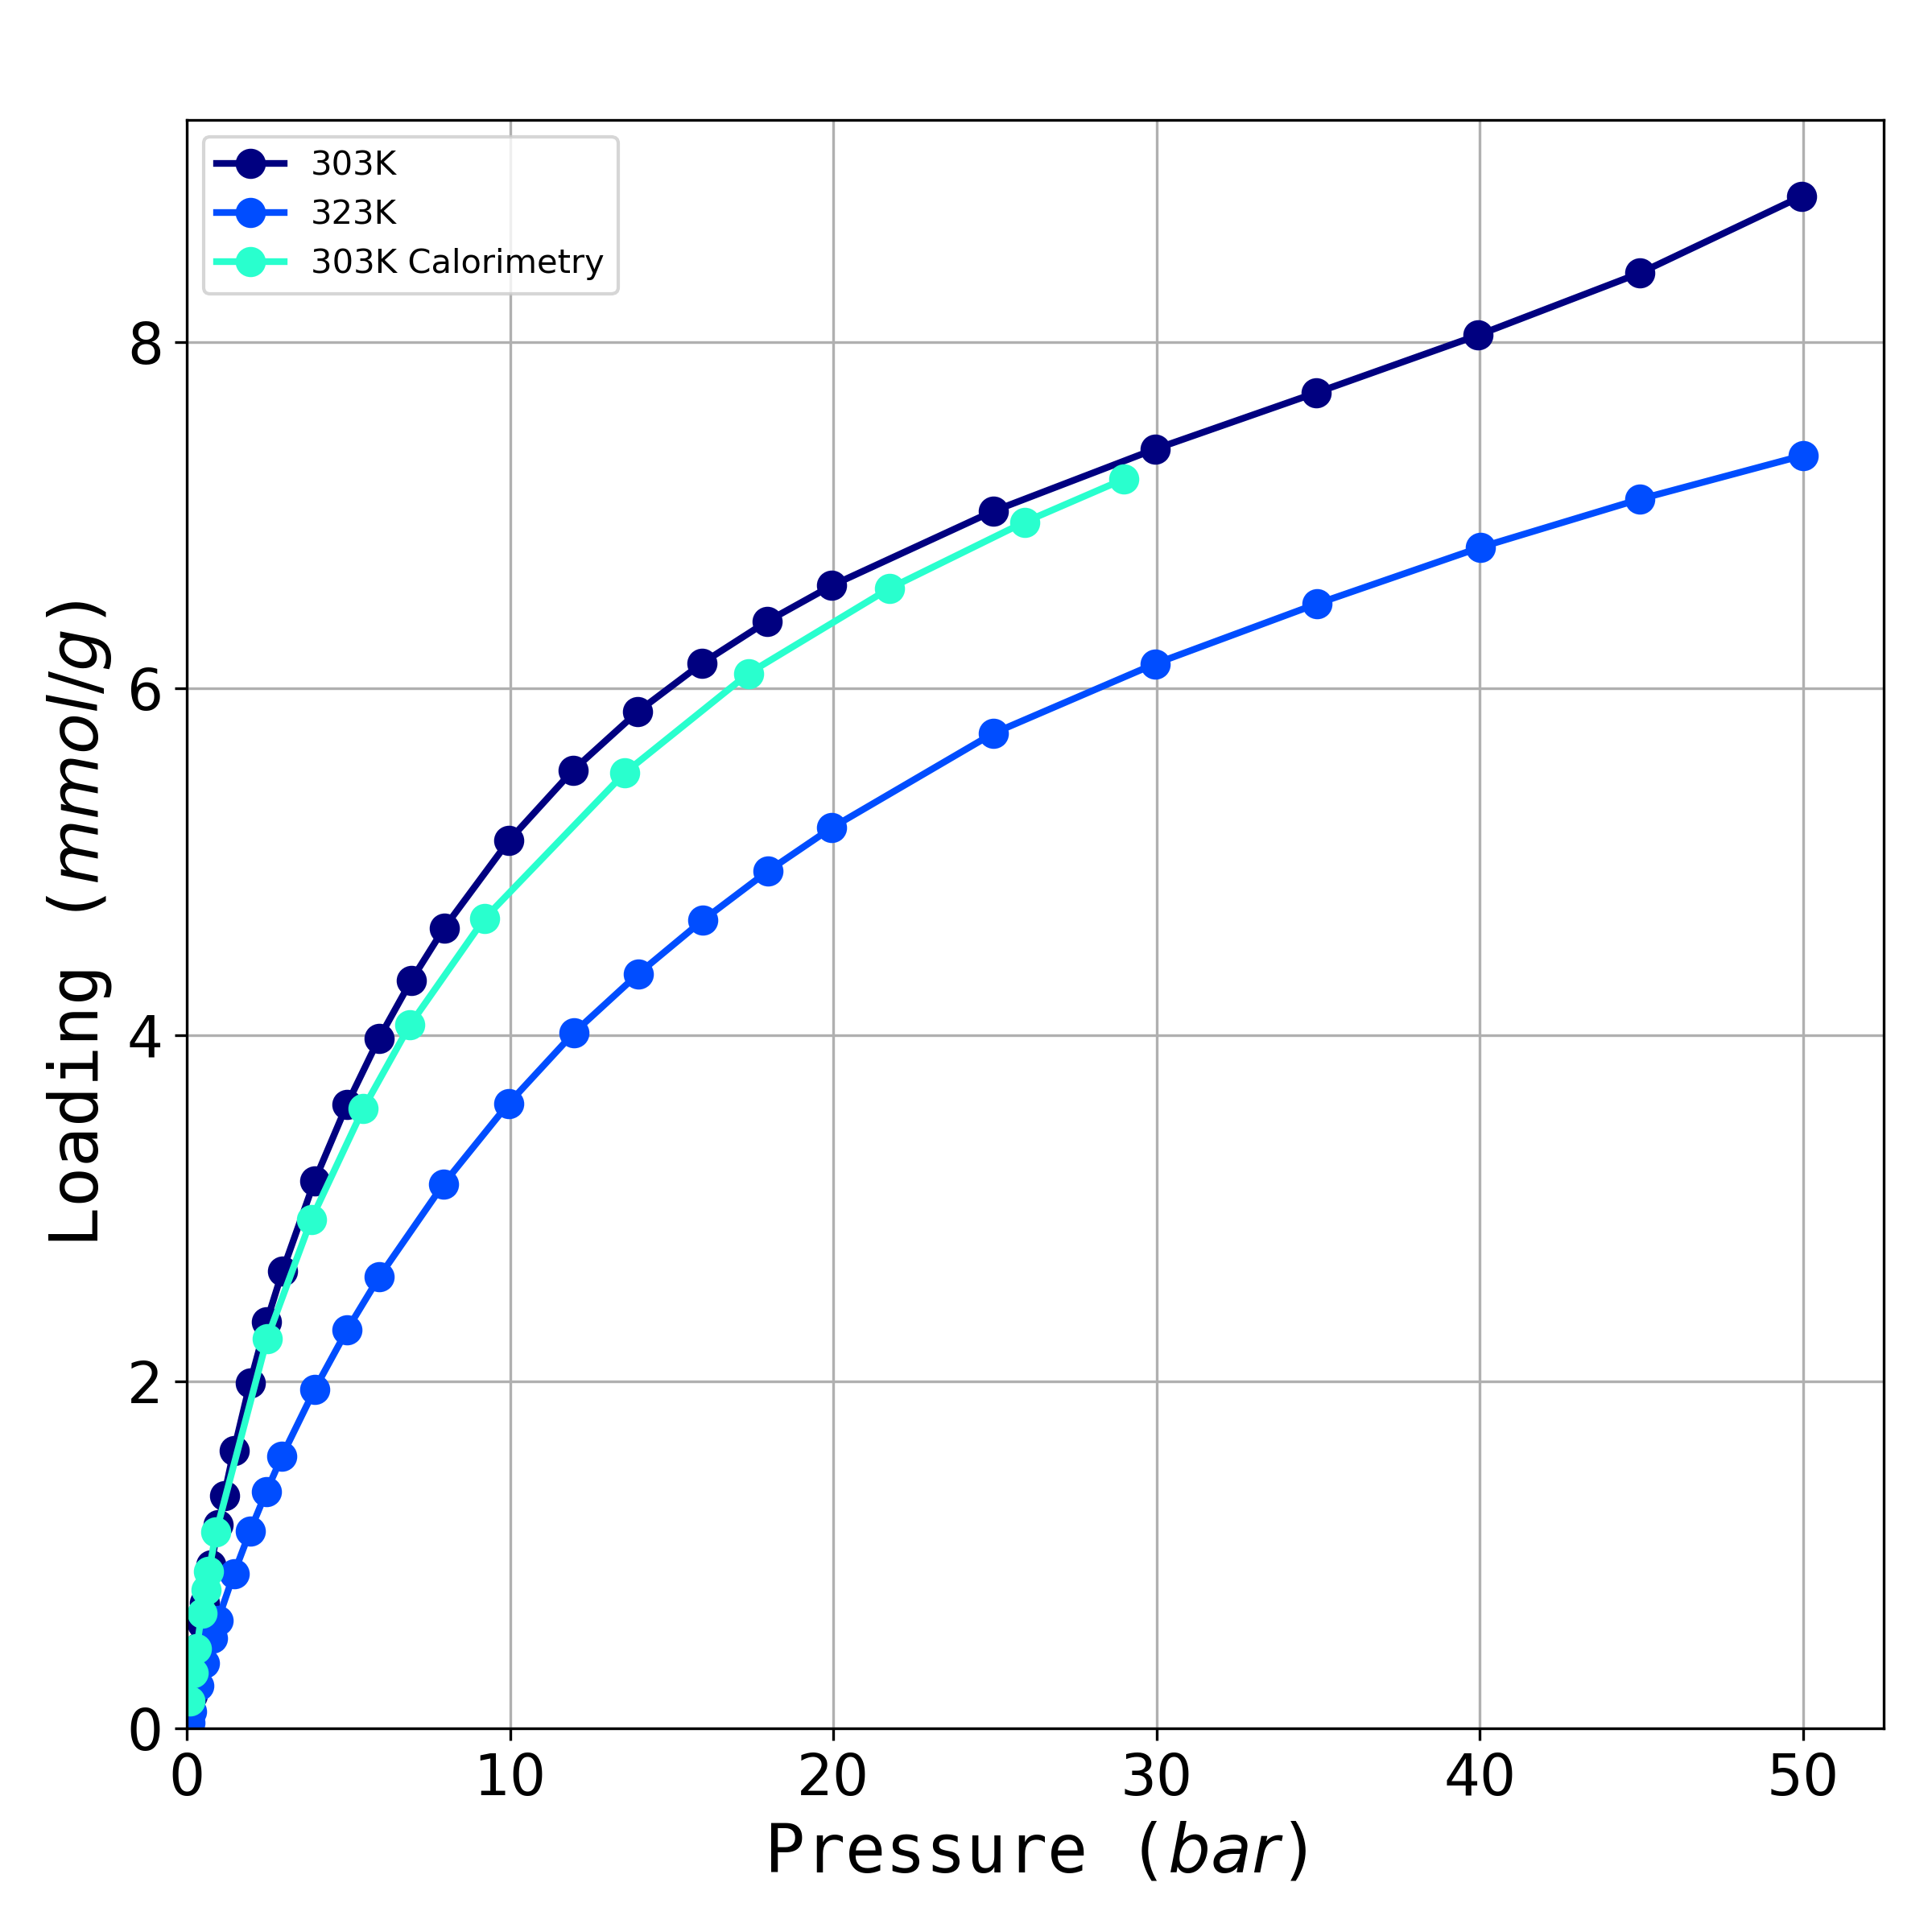
\includegraphics[width=.8\linewidth]{uio-isosteric-iso}
        \caption{}%
        \label{fig:uioisostericiso}
    \end{subfigure}%
    \begin{subfigure}[b]{.5\textwidth}
        \centering
        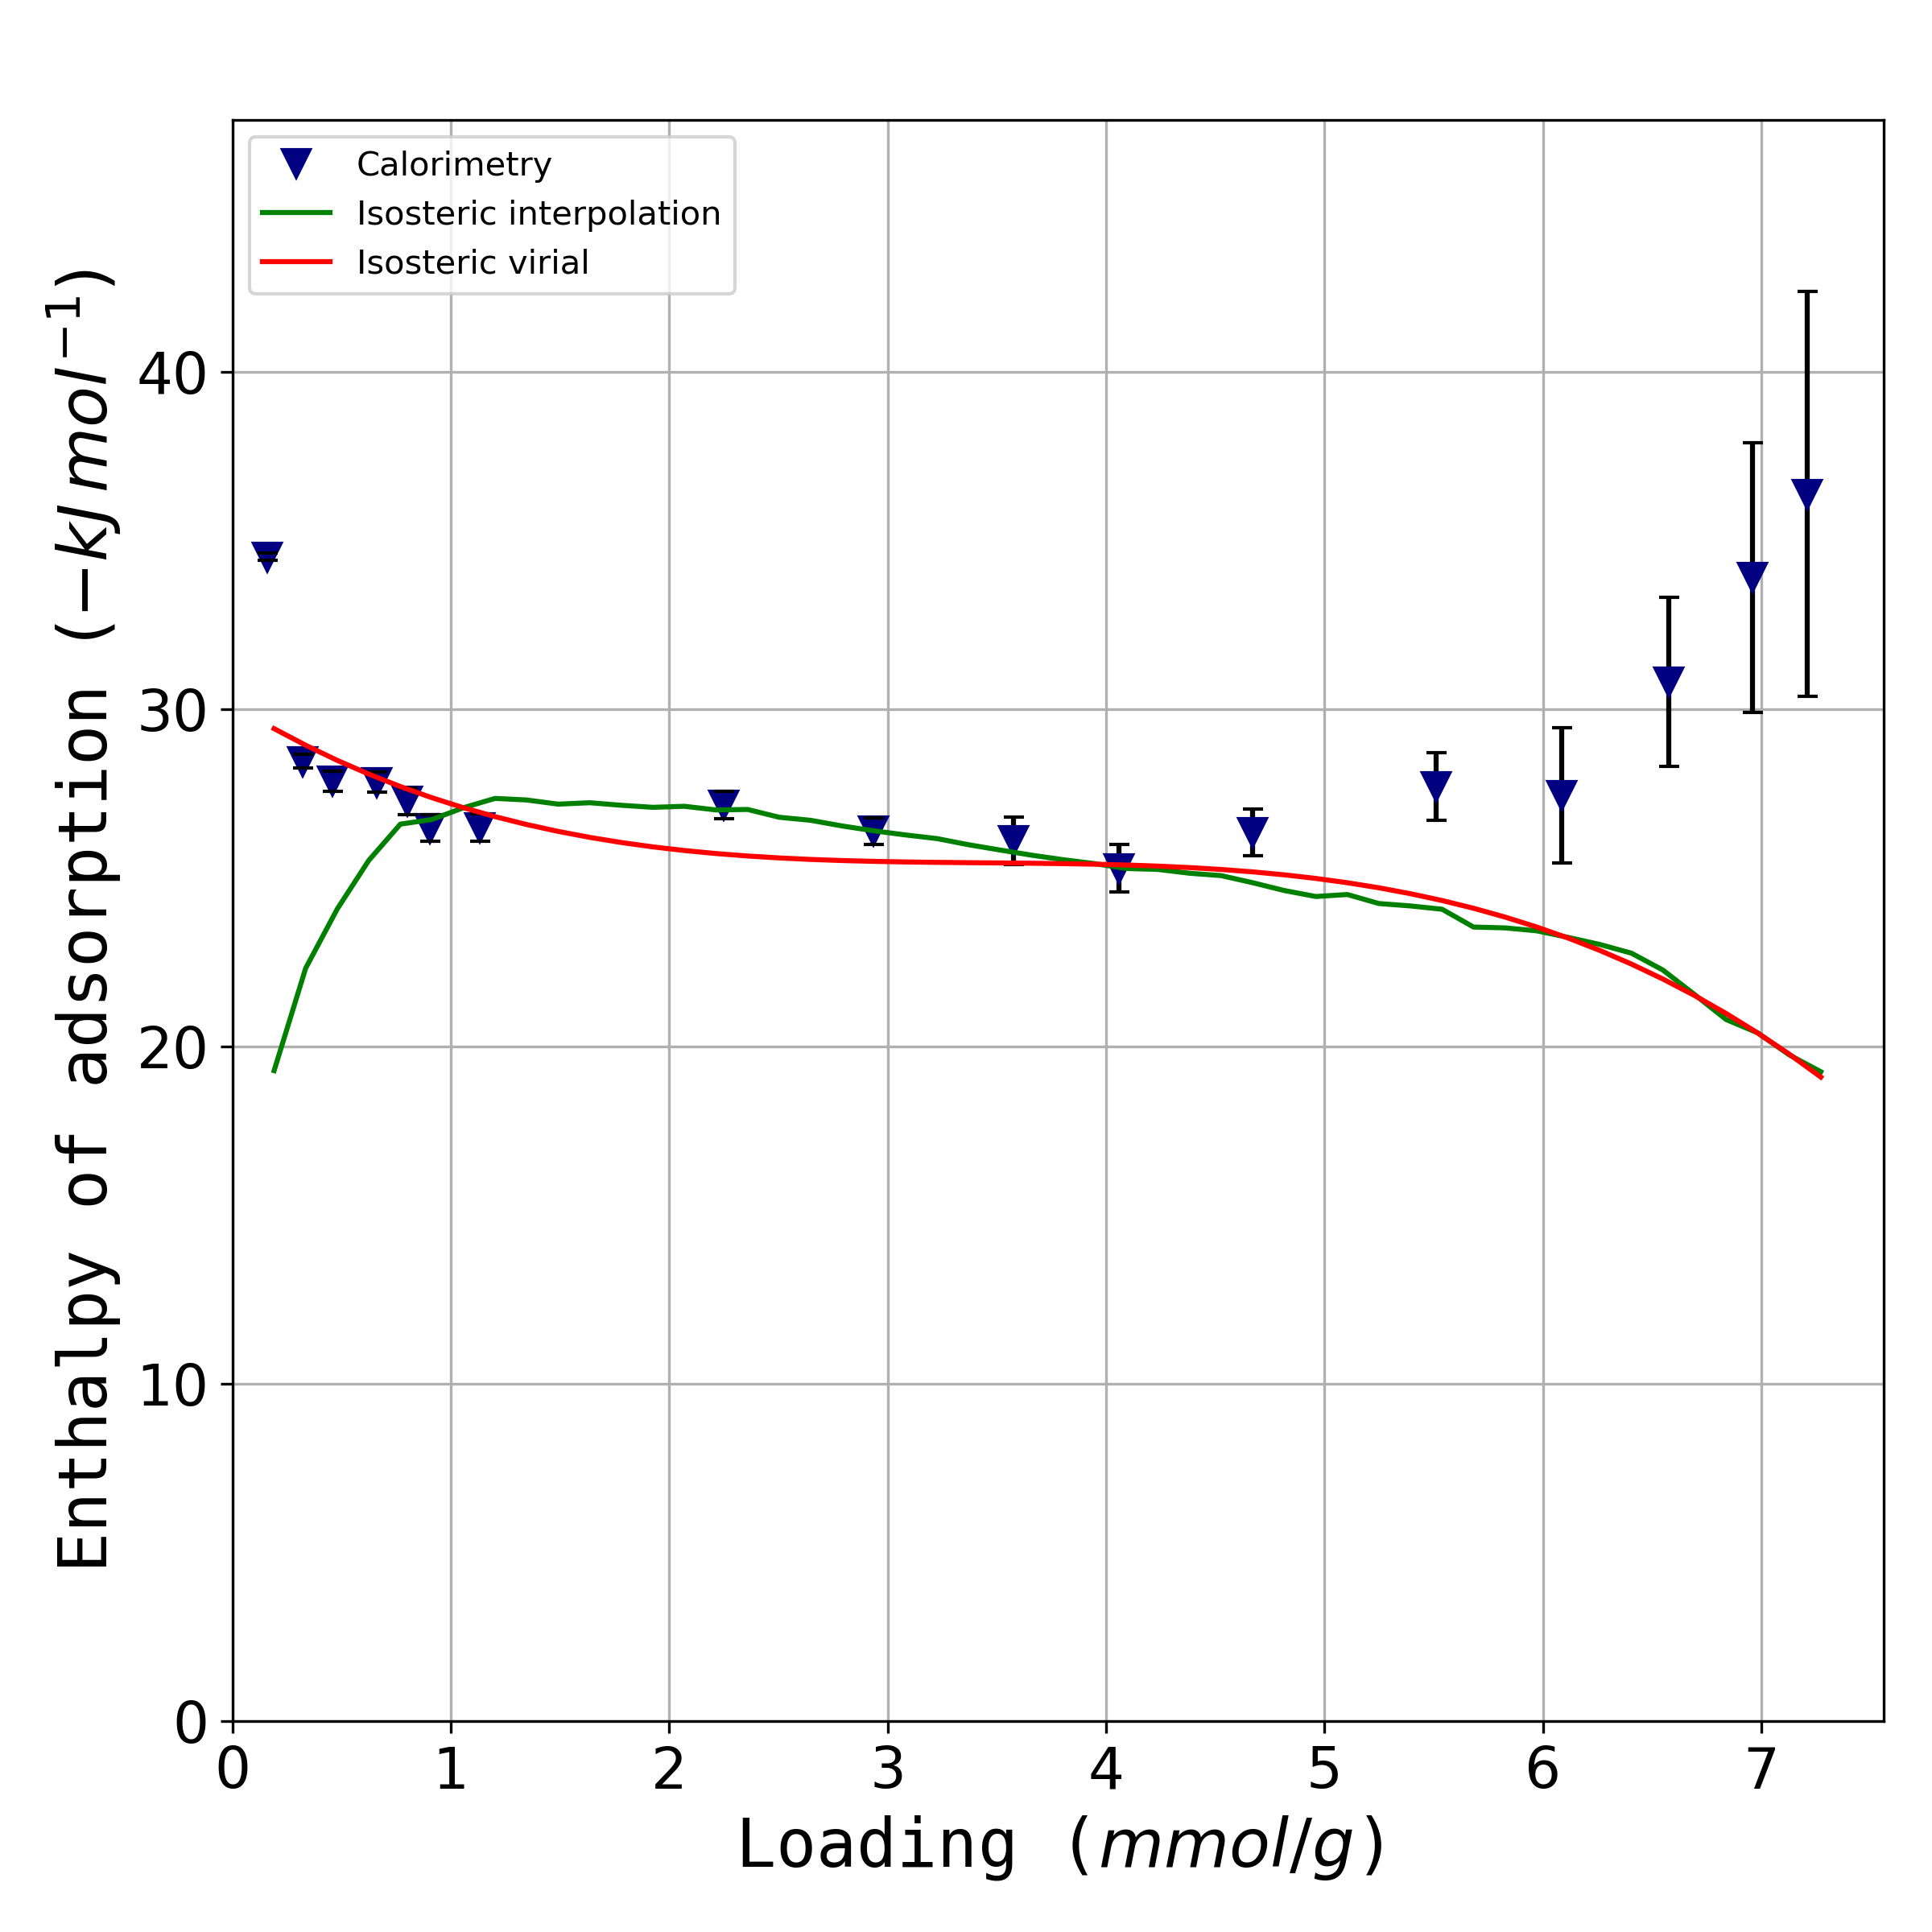
\includegraphics[width=.8\linewidth]{uio-isosteric-heat}
        \caption{}%
        \label{fig:uioisostericheat}
    \end{subfigure}
    \caption{Calculation of enthalpy of adsorption: (\protect\subref{fig:uioisostericiso}) 
    the dataset of isotherms used and (\protect\subref{fig:uioisostericheat}) the calculated
    isosteric heat (red line) together with the measured differential enthalpy of adsorption 
    (blue triangles)}%
    \label{fig:uioisosteric}

\end{figure}

\subsection{Analysis of a carbon sample for gas separation applications}

A sample of reference carbon Takeda 5A is to be investigated for an in-depth characterisation of
the adsorption behaviour of pure gases, with a focus on describing the pore environment.
Afterwards, the performance of different binary separations is evaluated, 
such as \ce{CO2}/\ce{N2} and propane/propylene.

Pure gas adsorption data has been recorded at \SI{303}{\kelvin} in conjunction with
microcalorimetry on \ce{N2}, \ce{CO}, \ce{CO2}, \ce{CH4}, \ce{C2H6},
\ce{C3H6} and \ce{C3H8}. The complete dataset is plotted with the 
\lstinline{pygaps.plot_iso()} function and can be seen in Figure~\ref{fig:takedadataset}.

Nitrogen and carbon monoxide are similar in their adsorption behaviour,
with a nearly linear isotherm and low capacities.
Hydrocarbons are adsorbed with higher loadings, with both propane and propylene 
reaching a plateau at low pressures. Propylene is seen to have a 
higher capacity than propane, with packing effects as a likely cause.
Carbon dioxide has the highest loading capacity of the entire dataset.

Two parameters can be useful in characterising the local pore environment before guest-guest
interactions come into effect: the Henry constant at low loadings as well as the initial 
enthalpy of adsorption. Both can be calculated with \texttt{pyGAPS}, with several options in 
regard to the methodology. Here, Henry's constant is calculated using the 
\lstinline{pygaps.initial_henry_virial()} function, which fits a virial model to 
the isotherm and then takes the limit at loading approaching zero. The initial enthalpy of
adsorption is obtained through the \lstinline{pygaps.initial_enthalpy_comp()} function.
This fits the enthalpy curve to a compound contribution from 
guest-host interaction, defects, guest-guest attraction and repulsion using a minimization 
algorithm. The results of the calculations are plotted versus the polarizability of the 
gas used, which can be obtained from the respective \texttt{Adsorbate} class.
Figure~\ref{fig:takedatrends} shows that both the parameters fall on a linear 
trend, which suggests that the interactions between those guests and the pore walls are 
mostly due to Lennard-Jones interactions. Carbon dioxide has a higher enthalpy 
of adsorption than the baseline due to the contribution from its quadrupole moment. 
There is almost a complete overlap between propane and propylene, which leads to
the conclusion that the unsaturated double bond does not interact in a specific way
with the carbon surface.
The difference between the two isotherms is due exclusively to steric and packing effects.

\begin{figure}[ht]

    \centering
    \begin{subfigure}[b]{.5\textwidth}
        \centering
        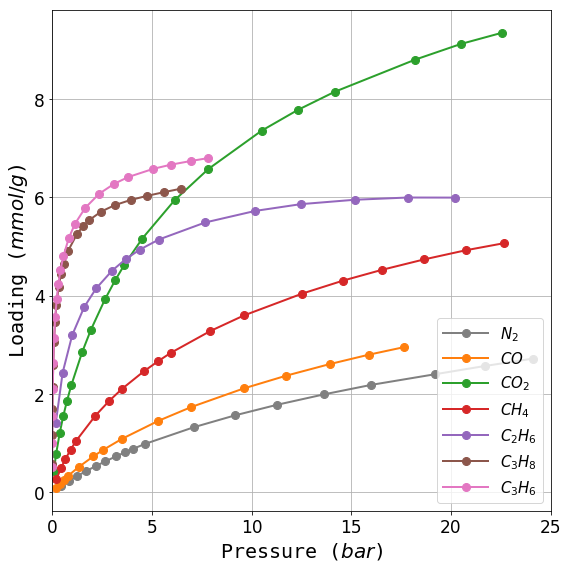
\includegraphics[width=.95\linewidth]{takeda-dataset}
        \caption{}%
        \label{fig:takedadataset}
    \end{subfigure}%
    \begin{subfigure}[b]{.5\textwidth}
        \centering
        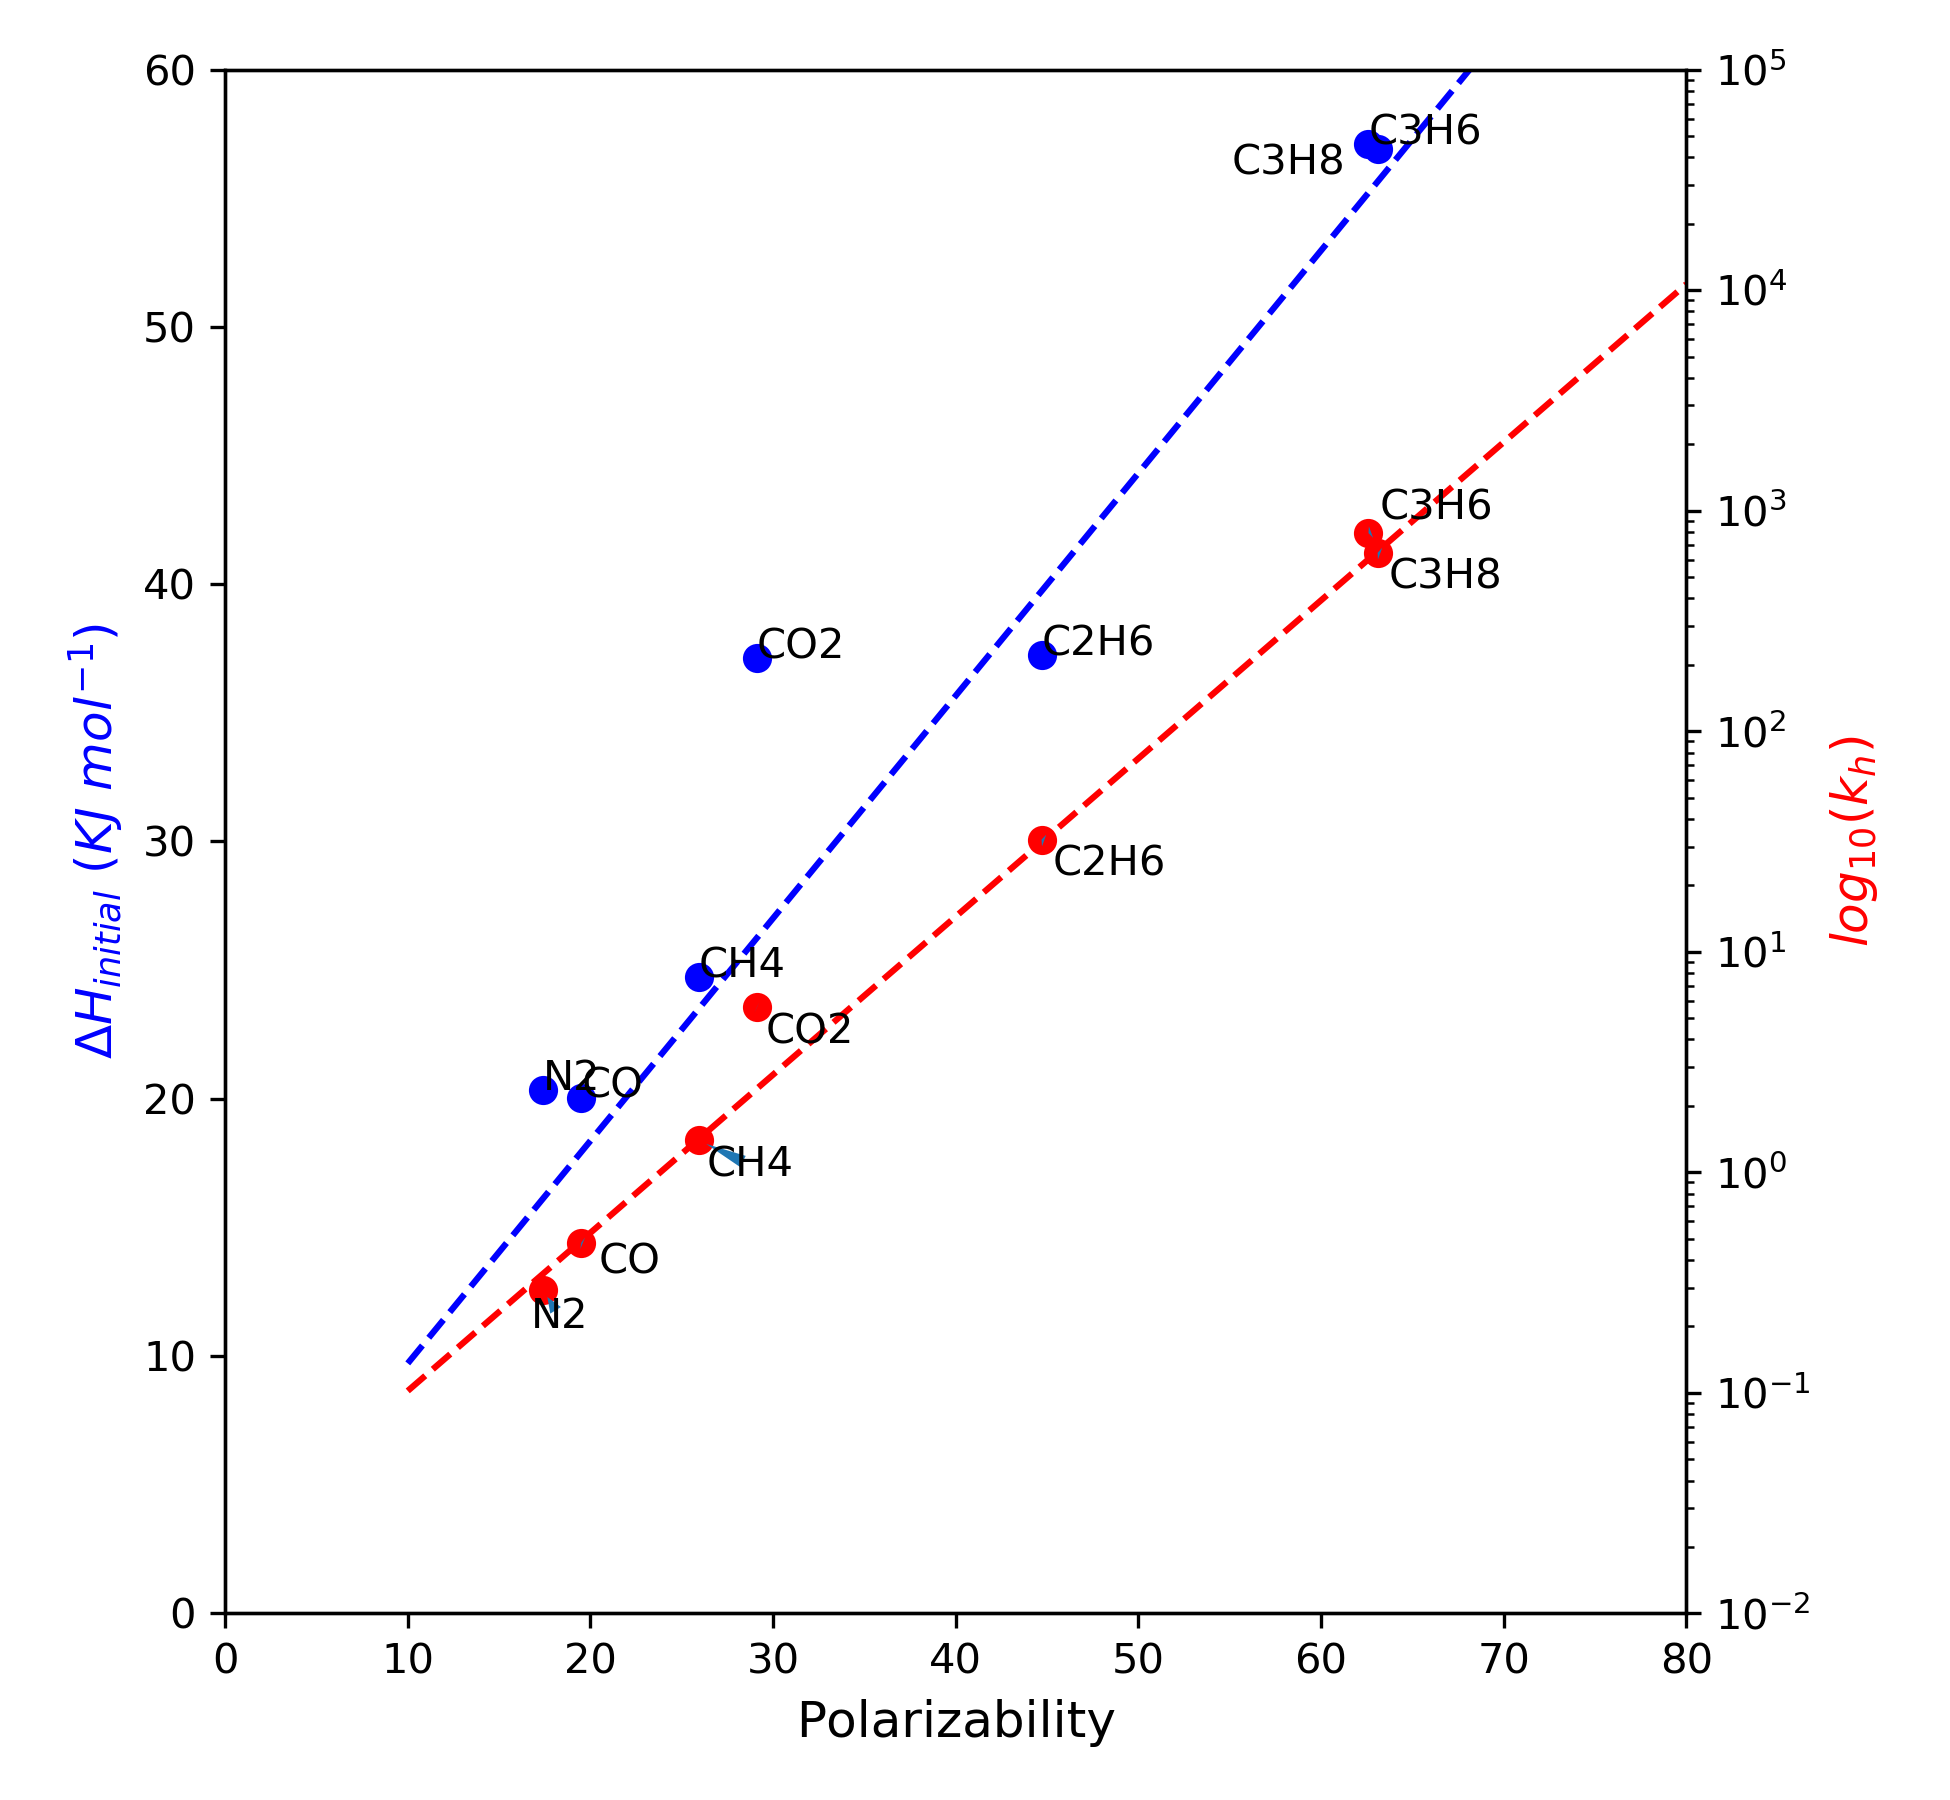
\includegraphics[width=.8\linewidth]{takeda-enth-henry}
        \caption{}%
        \label{fig:takedatrends}
    \end{subfigure}
    \caption{Takeda 5A dataset processing: (\protect\subref{fig:takedadataset}) the
    experimental dataset all recorded gases and (\protect\subref{fig:takedatrends}) the calculated
    trends of initial heat of adsorption and Henry's constant}%
    \label{fig:takedaanalysis}

\end{figure}

From the analysis of the pure gas dataset and the property-polarizability graph, two
potentially interesting separations arise, namely \ce{CO2}-\ce{N2} and 
propylene-propane. For these two pairs we use ideal adsorbed solution theory (IAST)
to simulate binary adsorption behaviour.
The \texttt{pyGAPS} framework includes a modified version of 
the pyIAST code~\cite{simonPyIASTIdealAdsorbed2016} which has been adapted to 
work with the \texttt{Isotherm} 
classes. Both model isotherms and real data can be used for IAST, with spreading 
pressure being calculated through the underlying isotherm model or through 
interpolation, respectively. Based on the previous analysis, we expect to see good 
performance for carbon
dioxide capture and little or no selectivity in the paraffin-olefin pair.

In this case, we fit the
experimental data to the available models in \texttt{pyGAPS}, then use the resulting model 
isotherms for IAST simulations. In order to get a `best-fit' model isotherm,
we use the function in Listing~\ref{lst:model},
which fits all available models and selects the one with the lowest 
residuals between the fitted function and the real data. Currently, the models available
in \texttt{pyGAPS} are: Henry, 
single, double and triple site Langmuir~\cite{langmuirAdsorptionGasesPlane1918a}, 
BET~\cite{brunauerAdsorptionGasesMultimolecular1938},
Quadratic~\cite{hillIntroductionStatisticalThermodynamics1986}, 
Jensen-Seaton~\cite{jensenIsothermEquationAdsorption1996}, 
Toth~\cite{tothUniformInterpretationGas},
Tempkin approximation~\cite{simonOptimizingNanoporousMaterials2014}, 
Virial~\cite{myersThermodynamicsAdsorptionPorous2002}, 
and the Flory-Huggins~\cite{cochranVacancySolutionTheory1985} and 
Wilson~\cite{suwanayuenGasAdsorptionIsotherm1980} variations of 
Vacancy Solution Theory (VST). 
The isotherms and their best-fitting model is displayed in Figure~\ref{fig:takedaco2n2iso}
for the \ce{CO2}-\ce{N2} pair and in Figure~\ref{fig:takedac3h6c3h8iso} for the 
\ce{C3H8}-\ce{C3H6} pair.

\begin{lstlisting}[caption={Guessing the best model},label={lst:model}]
model = pygaps.ModelIsotherm.from_pointisotherm(iso, guess_model=True)
\end{lstlisting}

For the carbon dioxide separation, we simulate all equilibrium points for the 
adsorbed and gaseous phases at different concentrations of the two gases at 1 bar.
To do this we use the \lstinline{pygaps.iast_vle()} function which produces an 
analogue of a vapour-liquid equilibrium at a specified pressure for a binary mixture.
The resulting graph of this function can be seen in Figure~\ref{fig:takedac3h6c3h8iast}.
As expected, the predicted adsorbed mixture is rich in carbon dioxide. Selectivity can
also be calculated in a single point, with the value at 15\% \ce{CO2} and \SI{1}{bar} 
being 16.5. 

\begin{figure}[h]

    \centering
    \begin{subfigure}[b]{.5\textwidth}
        \centering
        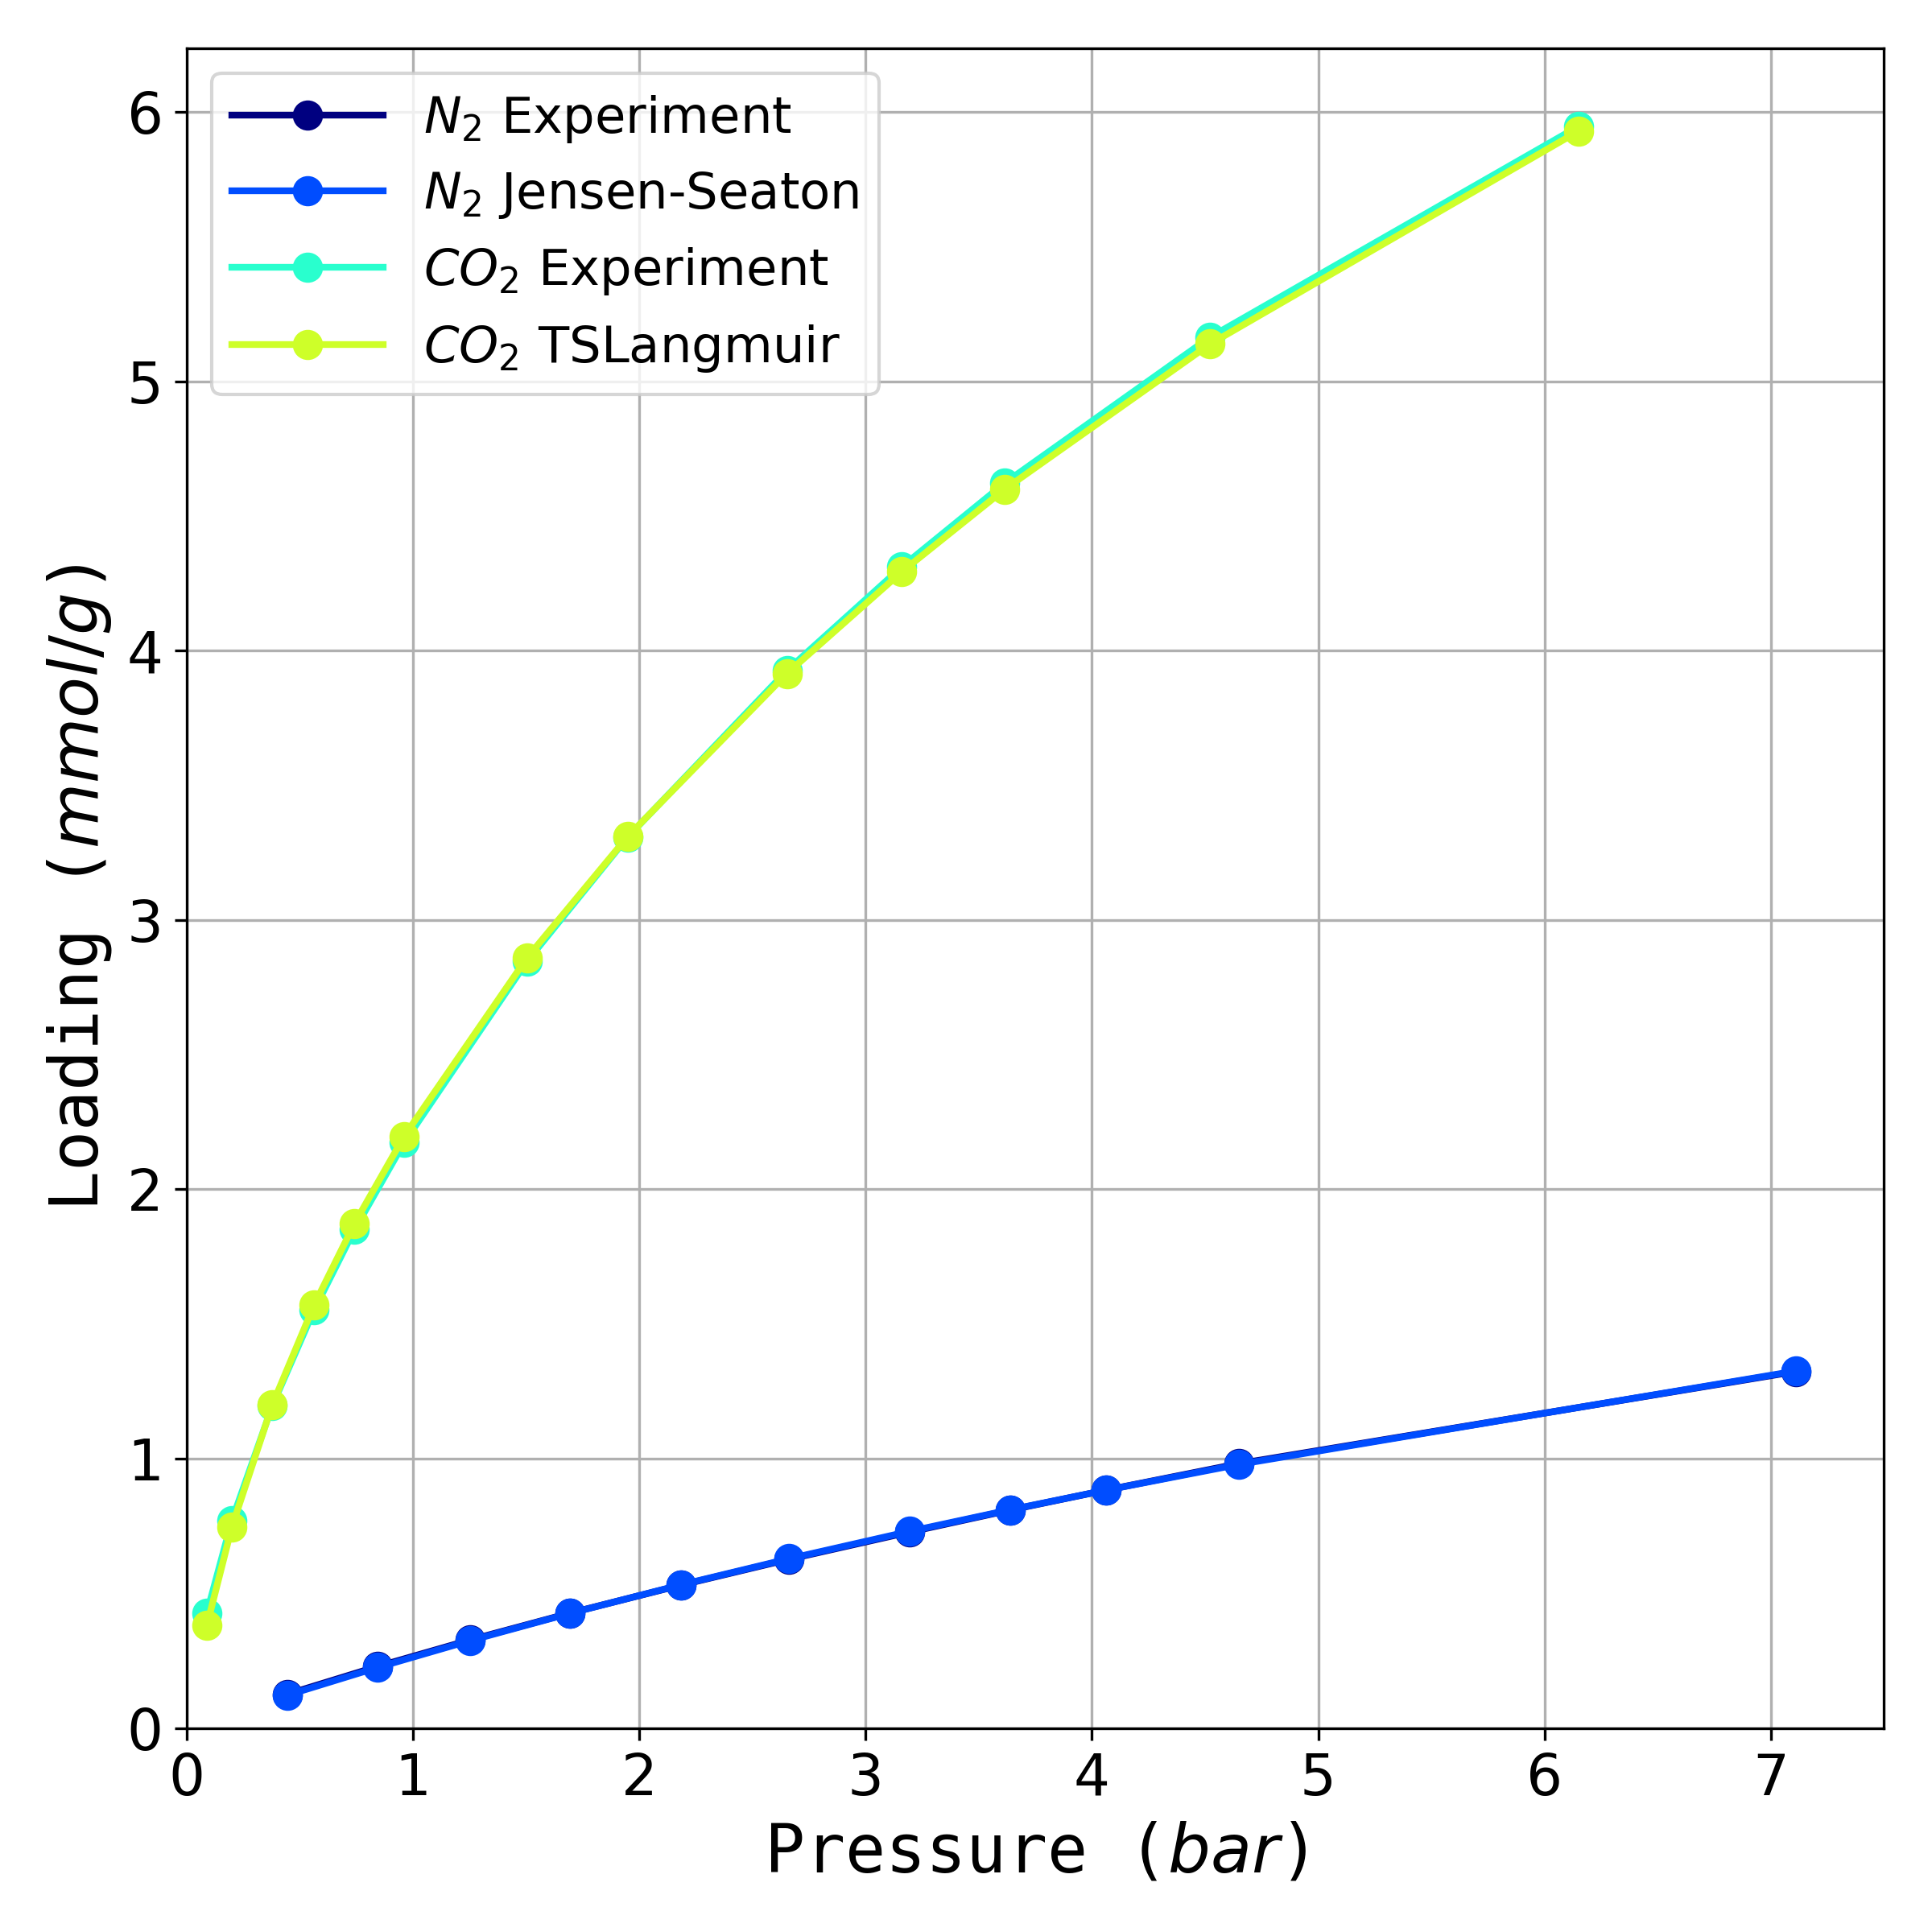
\includegraphics[width=.8\linewidth]{takeda-co2n2}
        \caption{}%
        \label{fig:takedaco2n2iso}
    \end{subfigure}%
    \begin{subfigure}[b]{.5\textwidth}
        \centering
        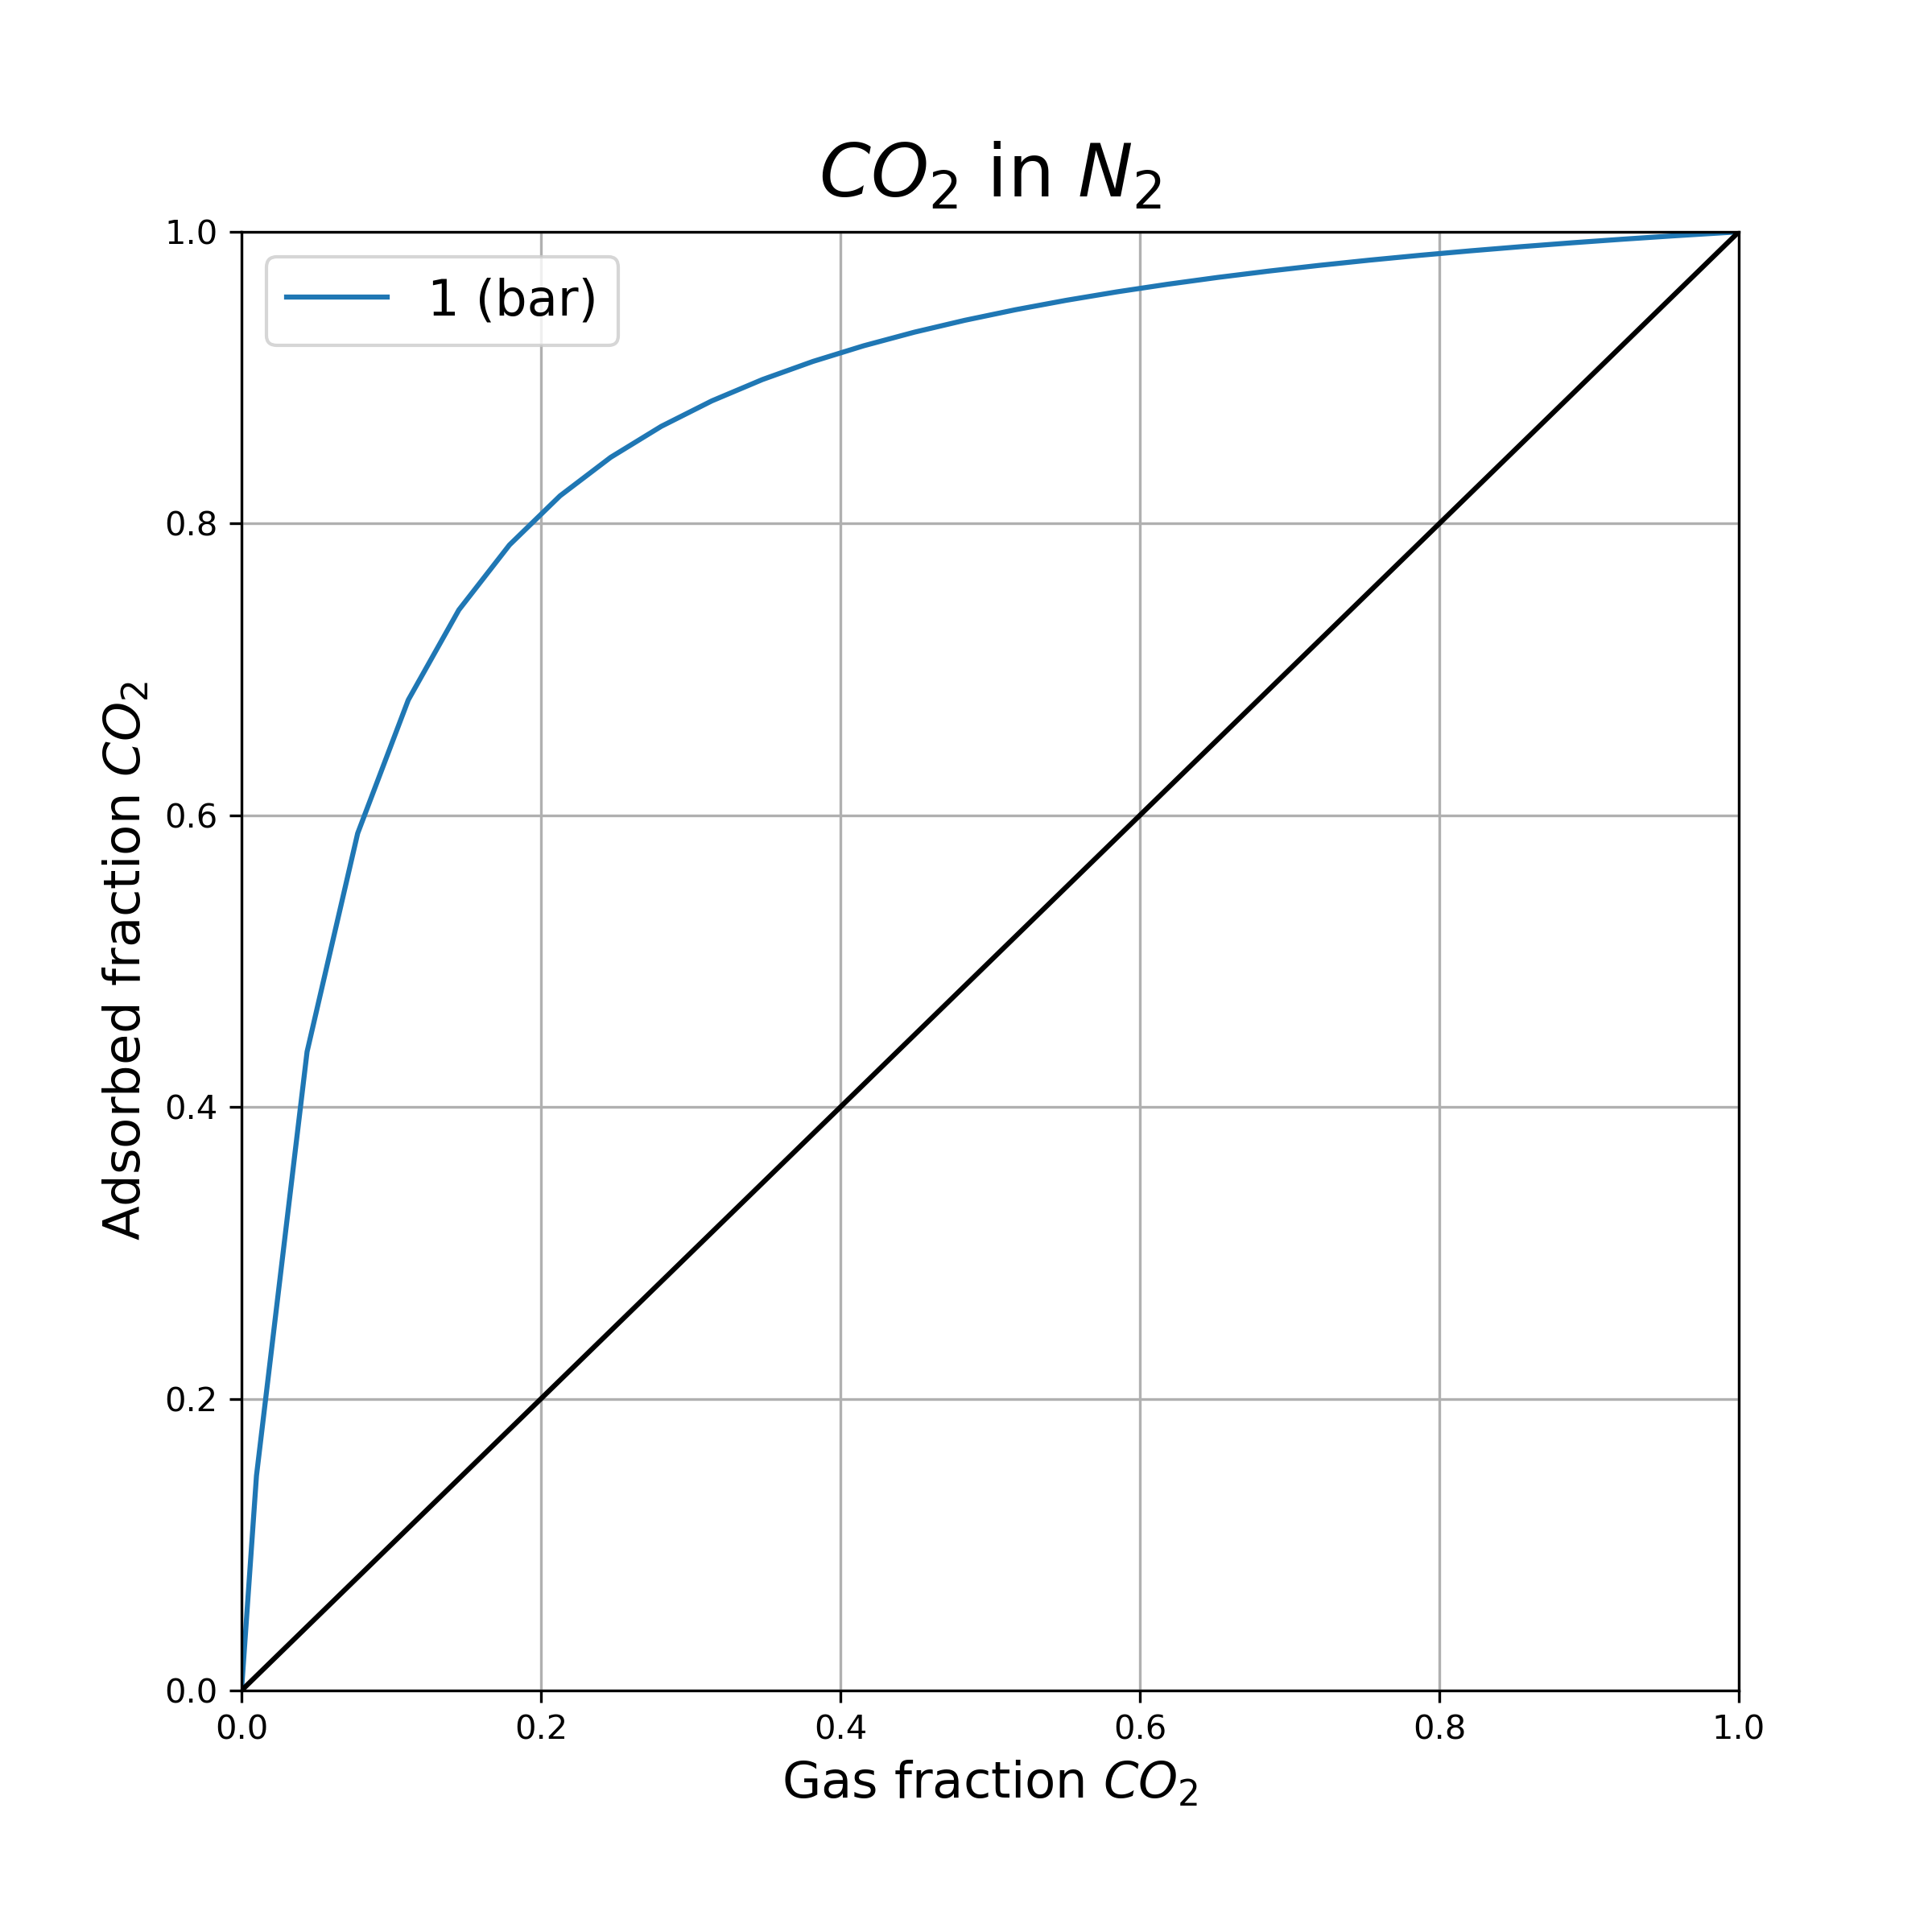
\includegraphics[width=0.92\linewidth]{takeda-co2n2-vle}
        \caption{}%
        \label{fig:takedaco2n2iast}
    \end{subfigure}
    \caption{Modelling binary adsorption of \ce{CO2} and \ce{N2}: 
    (\protect\subref{fig:takedaco2n2iso}) the pure component
    isotherms and their best fit models and (\protect\subref{fig:takedaco2n2iast}) 
    the predicted composition of the gaseous
    and adsorbed phase for different fractions of \ce{CO2} at \SI{1}{\bar}}%
    \label{fig:takedaco2n2}

\end{figure}

For the propane-propylene separation, we simulate the selectivity for propane
within a pressure range for a 50\% mixture of the two gases. It can be seen that
there is little or no preference for the unsaturated molecule, though the selectivity
increases slightly at pressures above \SI{1}{\bar}.

\begin{figure}[ht]

    \centering
    \begin{subfigure}[b]{.49\textwidth}
        \centering
        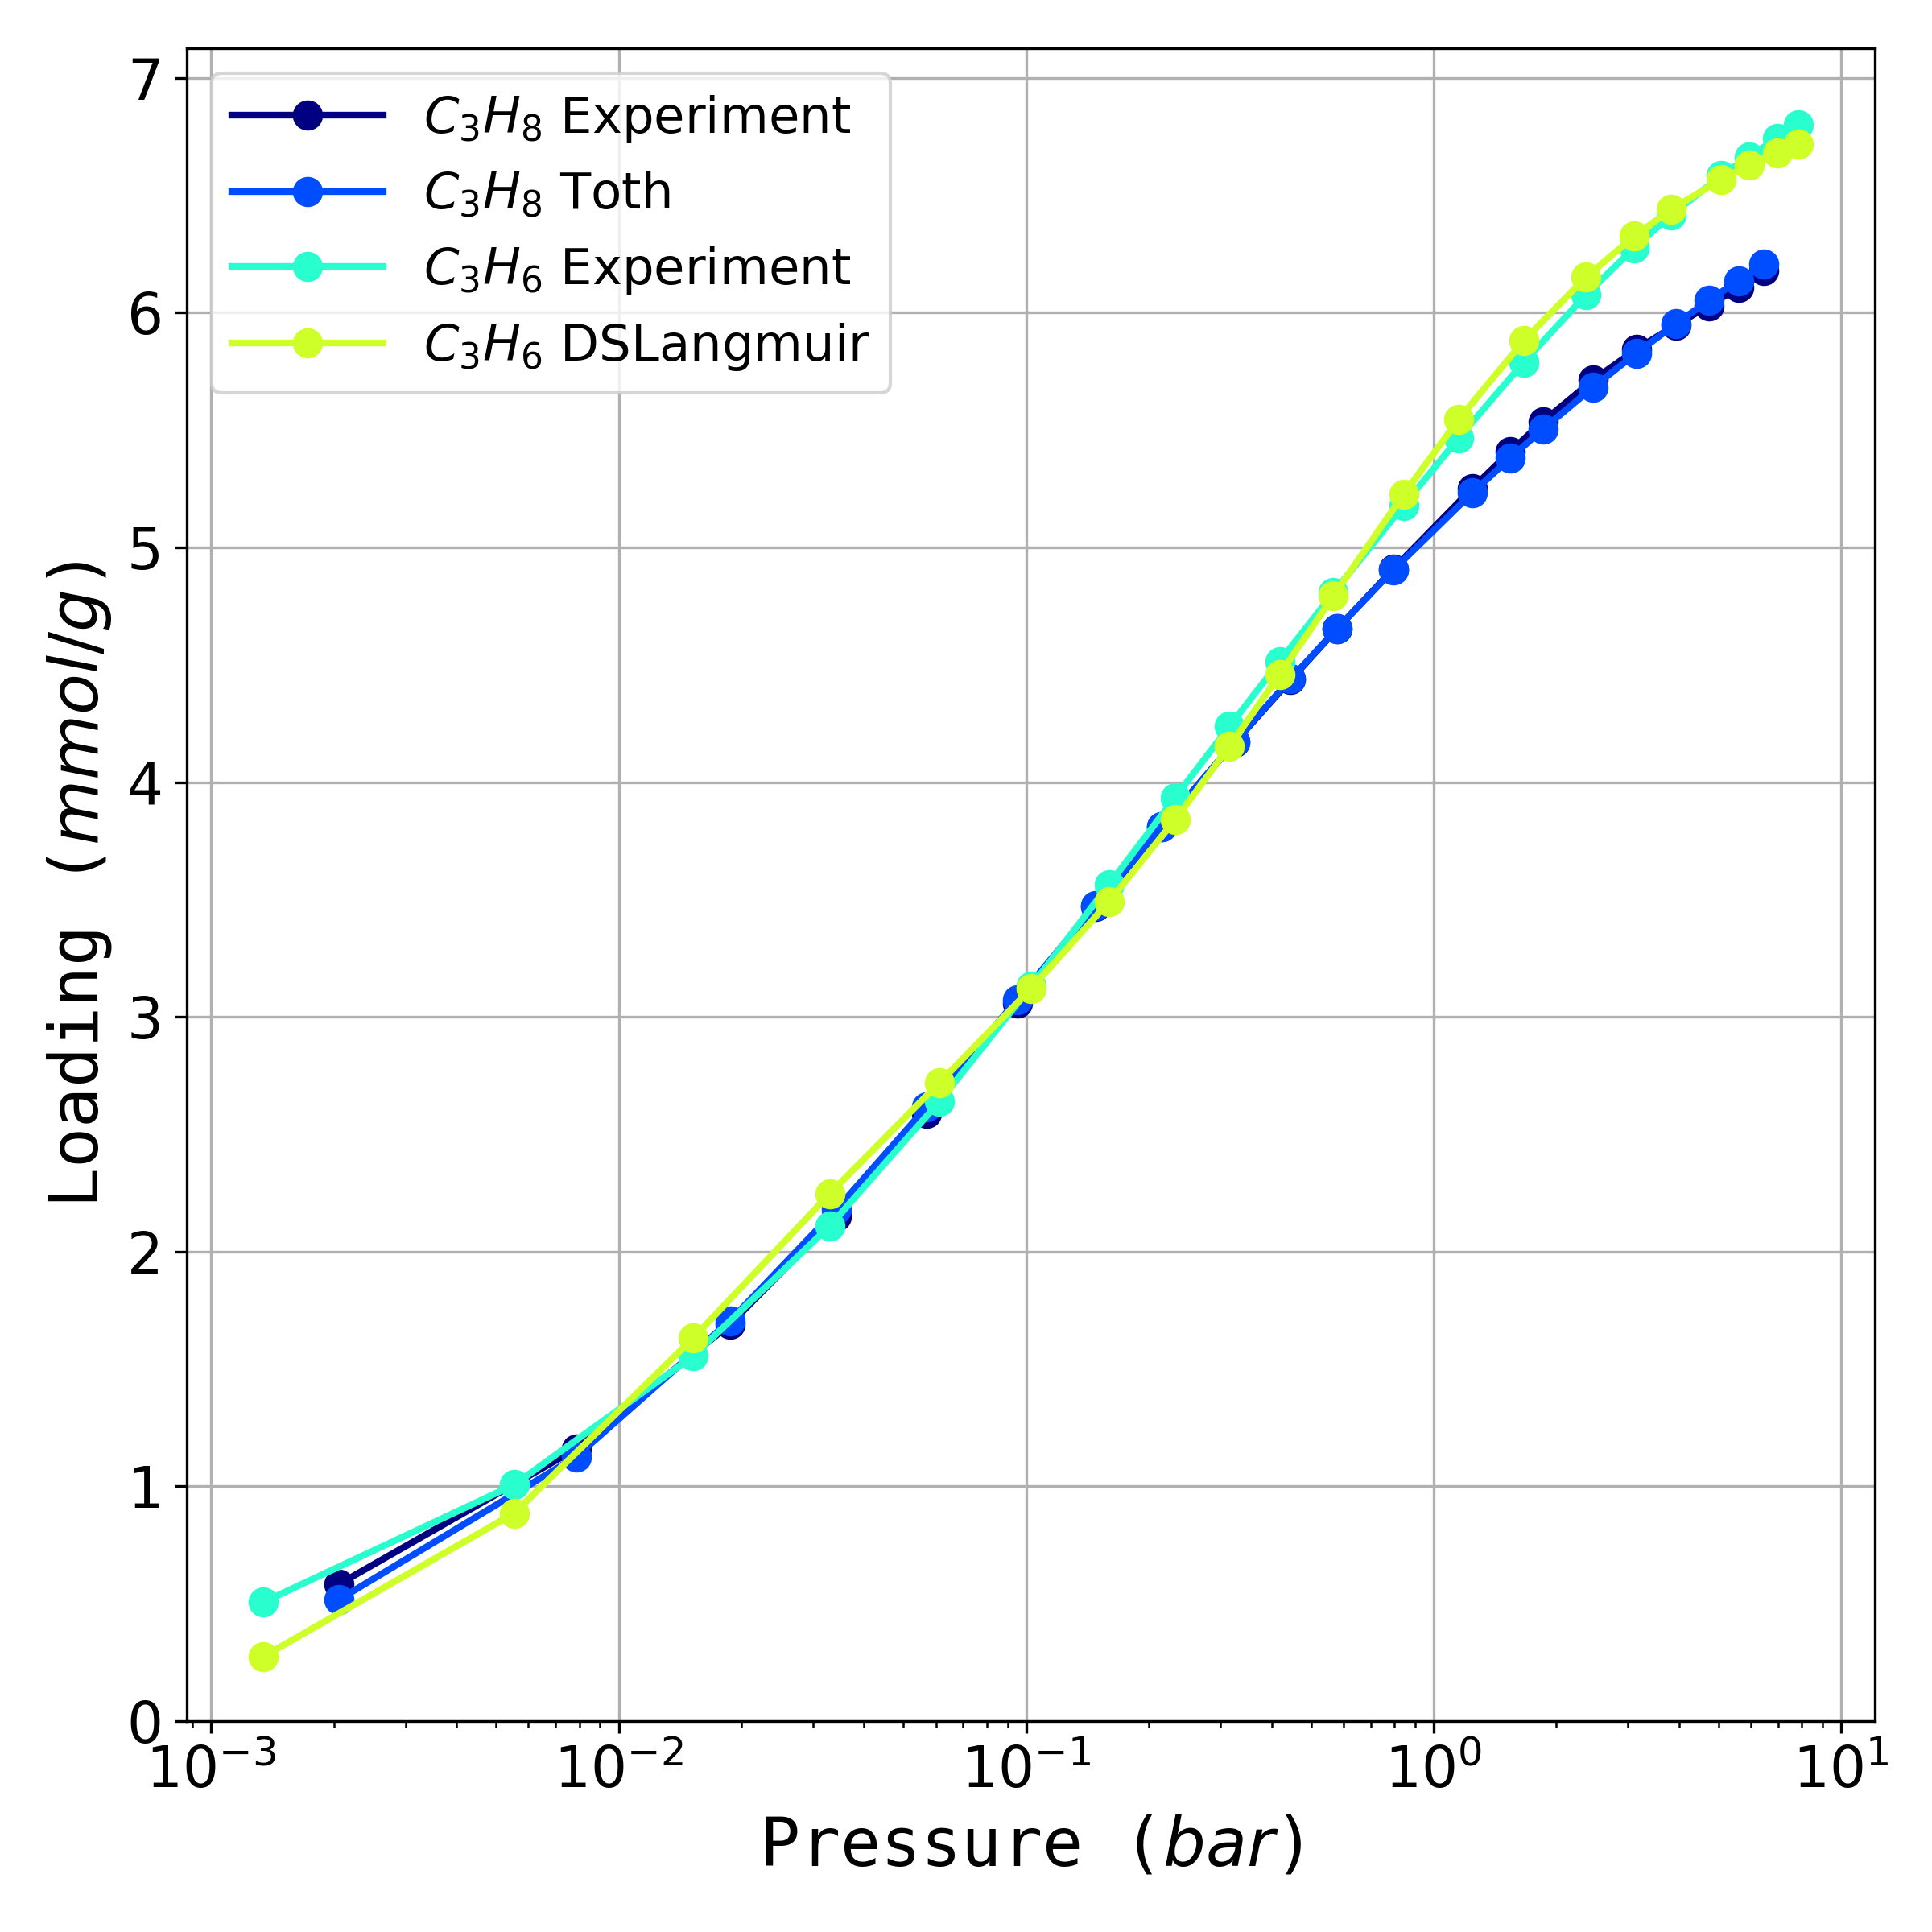
\includegraphics[width=.8\linewidth]{takeda-c3h6c3h8}
        \caption{}%
        \label{fig:takedac3h6c3h8iso}
    \end{subfigure}
    \begin{subfigure}[b]{.49\textwidth}
        \centering
        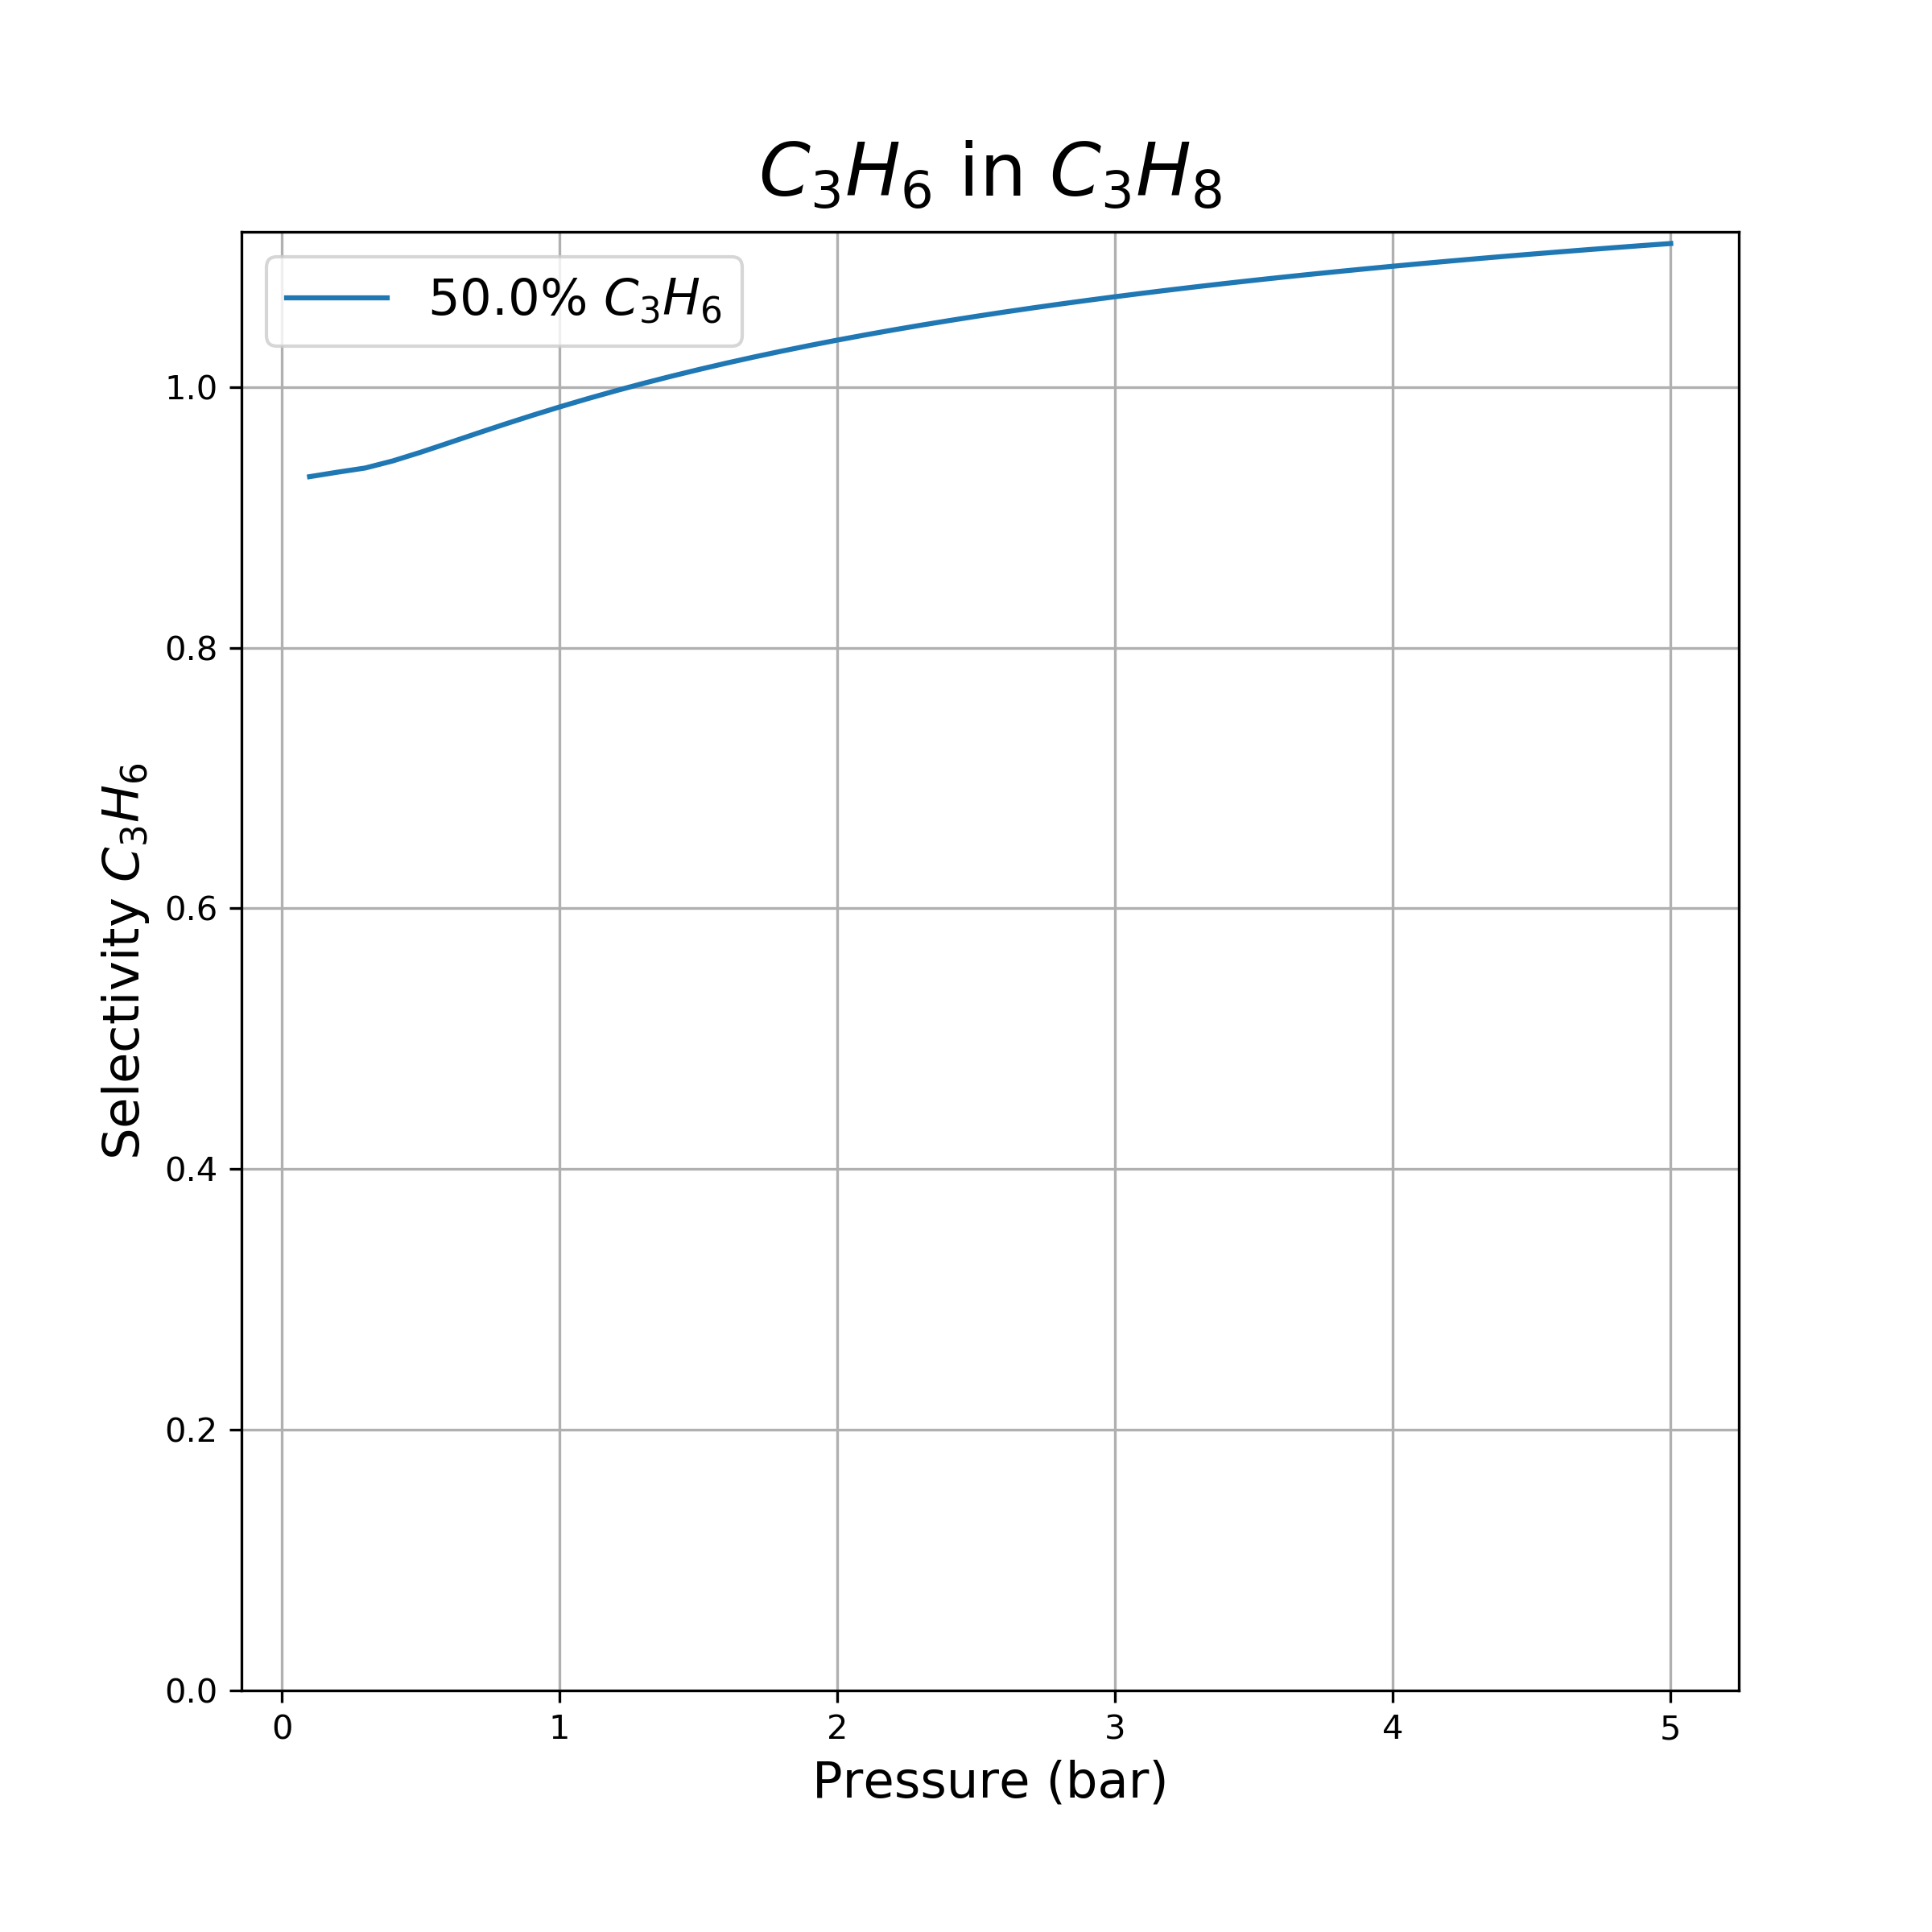
\includegraphics[width=.92\linewidth]{takeda-c3h6c3h8-svp}
        \caption{}%
        \label{fig:takedac3h6c3h8iast}
    \end{subfigure}
    \caption{Modelling binary adsorption of a propane-propylene mixture: 
    (\protect\subref{fig:takedac3h6c3h8iso}) the pure-component
    isotherms and their best fit models and (\protect\subref{fig:takedac3h6c3h8iast})
    the predicted selectivity of propane adsorption of a 50-50\% mixture in a range of 
    pressure from 0.1 to 7 bar}%
    \label{fig:takedac3h6c3h8}

\end{figure}